\documentclass[10pt]{article}
\usepackage[margin=1in]{geometry} 
\usepackage{amsmath,amsthm,amssymb, graphicx, multicol, array, graphicx, float, listings, csvsimple, longtable, booktabs}

\newcommand{\N}{\mathbb{N}}
\newcommand{\Z}{\mathbb{Z}}
    
\newenvironment{sect}[2][Section]{\begin{trivlist}
\item[\hskip \labelsep {\bfseries #2}]}{\end{trivlist}}

\begin{document}
    
\title{General Analysis on Loan Data}
\author{Nicholas Wan}
\maketitle

In this report, I will mainly discuss different features of 10000 granted loans in the past 5 years and whether these features have a positive or negative influence on the loans in terms of the status of the loans. In this experiment, we will be treating 10000 groups of loan data each consisting of 21 features and a status. By analyzing each feature, we will have a basic idea of the loans' performance.

\begin{sect}{Status Overview}
:\\
There are 7 possible status for each loan. Good loans are the ones where the status is current or fully paid. Bad loans are the ones where the status is default, in grace period or late. This graph below shows the general overview all loans in terms of their status.
\begin{center}
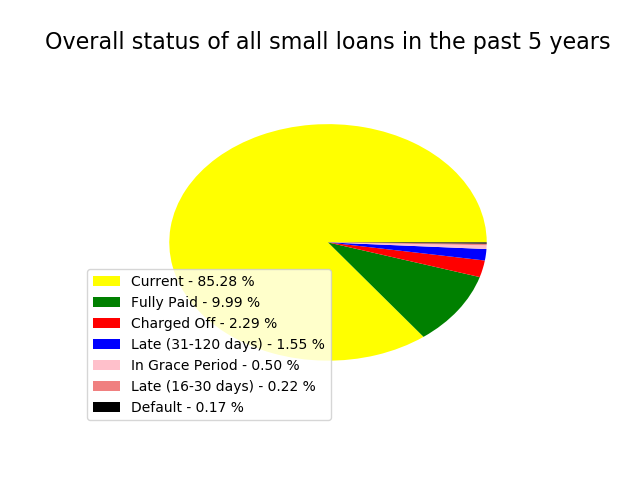
\includegraphics[scale=0.7]{overall_status_pie.png}
\end{center}
As we can see in this chart, good loans take up to $95.27\%$ out of all loans granted. It is safe to say that the company is in good shape. Now, let's dive deeper into the data and see if we can gain more information about how to improve the performance of the loans.
\end{sect}
\begin{sect}{Loan Amount}
:\\
First of all, let's see if the amount of each loan influences its status:\\
\begin{minipage}{0.5\textwidth}
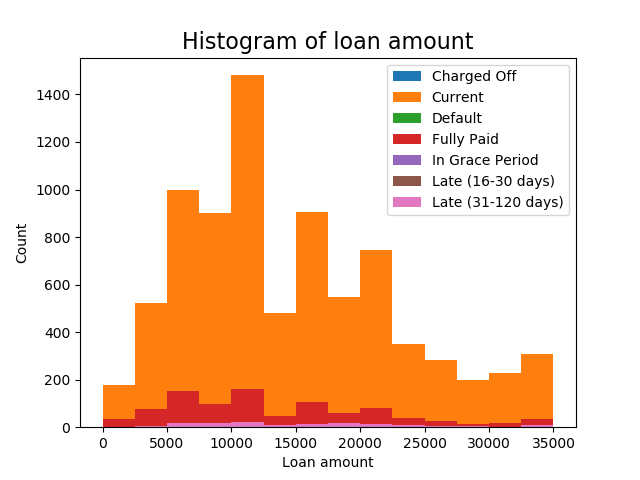
\includegraphics[width=\textwidth]{loan_amount_hist.png}
\end{minipage}
\begin{minipage}{0.5\textwidth}
In the histogram on the left, we can have a rough idea of the distribution of loan amount and the overall status among all loans. There are certain values that are more common than others. There are $720$ loans with amount equal to $10000$ and $304$ loans with amount equal to $35000$ .
\end{minipage}
% \includegraphics[scale=0.6]{}
% \begin{center}
\footnotesize\csvautobooktabular[/csv/respect all]{Loan_Amount_on_Status.csv}\\\\
\normalsize
The table above shows us the detail of the status of loans with different amount. For the sake of page space, I hide 3 columns in this table(Default, Late(31-120 days) and Late(16-30 days)). You are welcome to examine the file $Loan\_Amount\_on\_Status\_full.csv$ for full report.\\
In this table, each row indicates different loan amount interval represented by the left most column. The right most column indicates the good loan rate for that interval. We can see more clearly that most loans have the amount between $5,000$ to $25,000$ dollars. However, the good rate are similarly good among all intervals. As a result, for now we can conclude that the loan amount does not have major influence on loan status. Loans will not turn worse because of large amount or vice versa.

\end{sect}

\begin{sect}{Genral Purpose}
:\\
Now, we are going to analyze if the purpose of the loans have a major impact the loan status:\\
\begin{minipage}{0.5\textwidth}
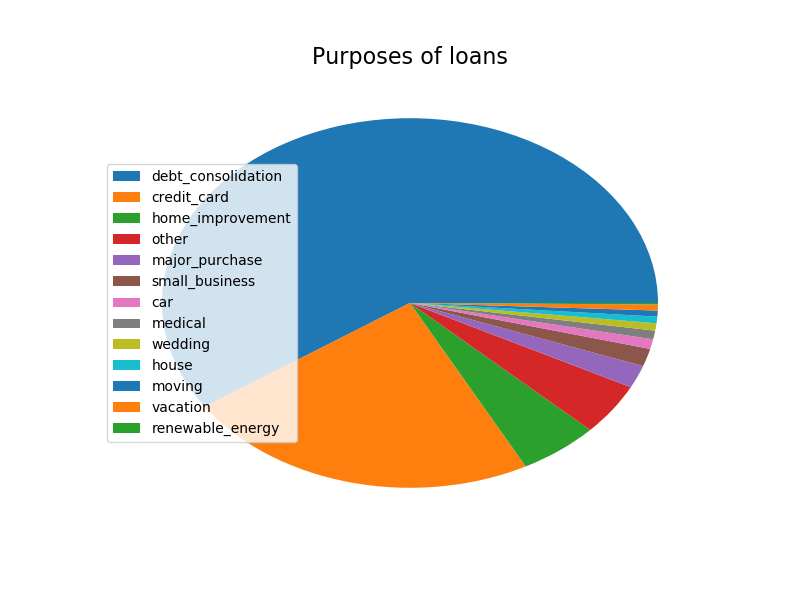
\includegraphics[width=\textwidth]{purpose_pie_chart.png}
\end{minipage}
\begin{minipage}{0.5\textwidth}
In the histogram on the left, we can have a rough idea of the distribution of general purpose of all the loans. As we can see, most of the loans are used for debt consolidation and credit card. These two purposes make up to 80\% of all loans. As a result, the good performance on loans with these two purpose will be significant to the good overall performance.
\end{minipage}
\begin{center}
\footnotesize\csvautobooktabular[/csv/respect all]{Purpose_on_Status.csv}\\
\end{center}
\normalsize
Now, let's get closer at each purpose to see their performance.\\
The table above shows us the detail of the status of loans with different purpose. For the sake of page space, I hide 3 columns in this table(Default, Late(31-120 days) and Late(16-30 days)). You are welcome to examine the file $Purpose\_on\_Status\_full.csv$ for full report.\\
First let's go to the two types of loans that care the most about: debt consolidation and credit card. Fortunately, they are both performing well with $95.06\%$ and $96.52\%$ good rate. If we want to improve the overall status on this two types, I reconmmand improving the loans with purpose of debt consolidation because its rate rate still has increasing space and it is the most common purpose of all.\\
Also, there are loans with certain purposes require our attention. Loans for small business have the worst good loan rate while its quantity is not small. As a result, this is a major draw-back in the overall status. Being more carefully in granting loans for small business will be a good choice in the future. Finally, loans for medical, renewable energy and wedding also need more careful examination in the future although they have relatively small amount.
\end{sect}

\begin{sect}{Interest Rate}
:\\
\begin{minipage}{0.5\textwidth}
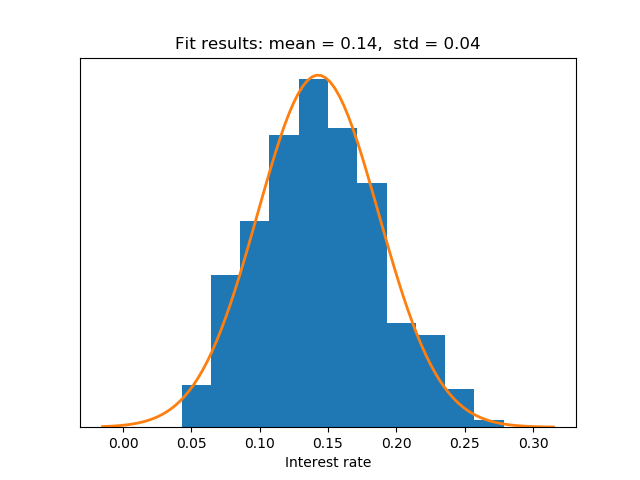
\includegraphics[width=\textwidth]{intrate_hist.png}
\end{minipage}
\begin{minipage}{0.5\textwidth}
In the histogram on the left, we can have a rough idea of the distribution of the interest rate of all the loans. As we can see, the interest rate are normally distributted and therefore we fit a normal distribution onto our data. Our distribution has $mean=0.14$ and $\text{standard deviation}=0.04$. In general, our distribution is performing good in predicting interest rate for a single loan.
% TODO Figure out fitting normal distribution on interest rate hist.    
\end{minipage}
\begin{center}
\footnotesize\csvautobooktabular[/csv/respect all]{Interest_Rate_on_Status.csv}\\
\end{center}
\normalsize
Furthermore, we are going to analyze the performance of loans in different interest rate interval according to table above. For the sake of page space, I hide 3 columns in this table(Default, Late(31-120 days) and Late(16-30 days)). You are welcome to examine the file $Interest\_Rate\_on\_Status\_full.csv$ for full report.\\
In this table, different rows represent different interest rate interval indicated by the left most column and the right most column tells us the good loan rate for that interval. Starting from 0.06 up to 0.28, we can observe that no whether the amount of loans in the intervals are small or big, the good loan rate is constantly decreasing.\\
As a result, I believe it is safe to conclude that the higher the interest rate of one loan is, the bigger risk there is for that loan to turn bad.

\end{sect}

\begin{sect}{Conclusion}
:\\
Based on my evidence and analysis above, there are several conclusions that I can safely draw from the data sample:
\begin{enumerate}
\item[I)] The status of all loans is generally good and good loans(current of fully paid) make up $95.27\%$ of all loans;
\item[II)] Loan amount do not have major impact on loan status. Loans have stable performance with small or large amount;
\item[III)] Loans that are used for debt consolidation make up the majority of all loans and loans that are used for debt consolidation or credit card make up to over $80\%$ of all loans;
\item[IV)] Loans that are used for small business perform the worst among all loans;
\item[V)] Loans that used for renewable energy, medical or wedding perform poorly but with fairly small amount;
\item[VI)] The interest rate of all loans are normally distributed with approximately $mean = 14\%$ and $std = 0.04$;
\item[VII)] The higher the interest rate is, the worse the loan is likely to perform.
\end{enumerate}

\end{sect}

% \csvautobooktabular[/csv/respect all]{test.csv}
% \begin{left}
% \tiny\csvautobooktabular[/csv/column names=C & F & C-OFF & LL & G & LS & D & Sum & Good & Bad & G Rate]{Loan_Amount_on_Status.csv}
% \end{left}

\end{document}